%%%%%%%%%%%%%%%%%%%%%%%%%%%%%%%%%%%%%%%%%%%%%%%%%%%%%%%%%%%%%%%%%%%%%%%%%%
%%%%%                         CHAPITRE 3                            %%%%%%
%%%%%%%%%%%%%%%%%%%%%%%%%%%%%%%%%%%%%%%%%%%%%%%%%%%%%%%%%%%%%%%%%%%%%%%%%%

\lhead[\fancyplain{}{\leftmark}]%Pour les pages paires \bfseries
      {\fancyplain{}{}} %Pour les pages impaires
\chead[\fancyplain{}{}]%
      {\fancyplain{}{}}
\rhead[\fancyplain{}{}]%Pour les pages paires 
      {\fancyplain{}{\rightmark}}%Pour les pages impaires \bfseries
\lfoot[\fancyplain{}{}]%
      {\fancyplain{}{}}
\cfoot[\fancyplain{}{\thepage}]%\bfseries
      {\fancyplain{}{\thepage}} %\bfseries
\rfoot[\fancyplain{}{}]%
     {\fancyplain{}{\scriptsize}}


%%%%%%%%%%%%%%%%%%%%%%%%%%%%%%%%%%%%%%%%%%%%%%%%%%%%%%%%%%%%%%%%%%%%%%%%%%
%%%%%                      Start part here                          %%%%%%
%%%%%%%%%%%%%%%%%%%%%%%%%%%%%%%%%%%%%%%%%%%%%%%%%%%%%%%%%%%%%%%%%%%%%%%%%%

\chapter{A practical implementation: the Pose2Sim Python package}
\label{ch:3}

%==============================================================================	Résumé du chapitre

\begin{center}
\rule{0.7\linewidth}{.5pt}
\begin{minipage}{0.7\linewidth}
\smallskip

\textit{ Sport scientists would benefit from having access to a user-friendly integrated workflow for on-field analysis. We propose the Pose2Sim open-source python package, as an alternative to the more usual marker-based motion capture methods. Pose2Sim stands for "OpenPose to OpenSim", as it uses OpenPose inputs (2D keypoints coordinates obtained from multiple videos) and leads to an OpenSim result (physically consistent full-body 3D joint angles). Code is available at \url{https://github.com/perfanalytics/pose2sim}. \newline \newline
This chapter is adapted from the article published in the Journal of Open Source Software: "Pose2Sim: An Open-source Python Package for multiview markerless kinematics" \cite{Pagnon2022b}. See Figure~\ref{fig_visabstract1} for a visual abstract.}

%\smallskip
\end{minipage}
\smallskip
\rule{0.7\linewidth}{.5pt}
\end{center}

\pagebreak
\minitoc

\vspace*{3cm}

\begin{figure}[hbtp]
	\centering
	\def\svgwidth{1\columnwidth}
	\fontsize{10pt}{10pt}\selectfont
	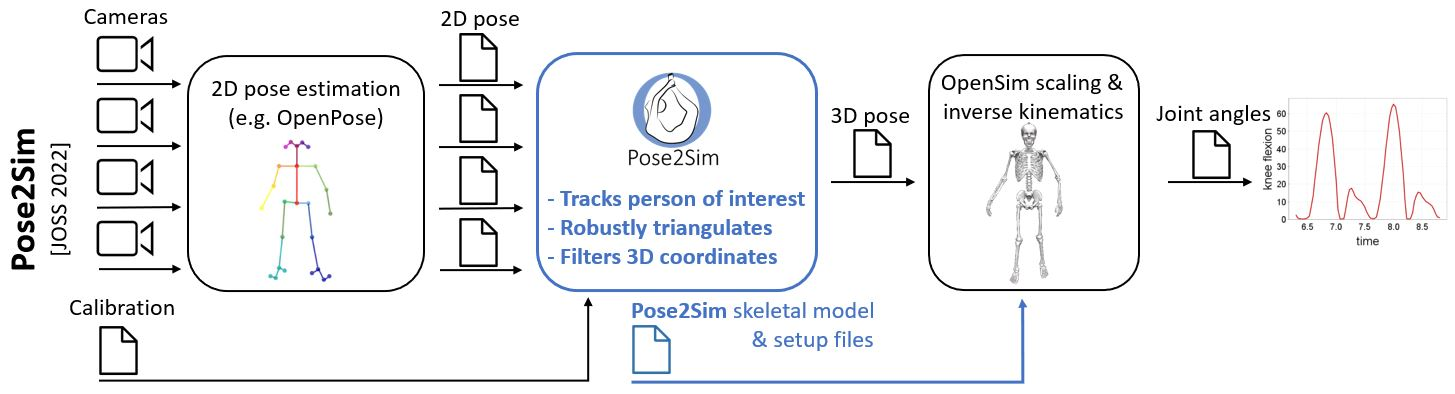
\includegraphics[width=\linewidth]{"../Intro/Figures/Fig_VisAbstract1.JPG"}
      \caption{Visual abstract for the Pose2Sim workflow \cite{Pagnon2022b}.}
	\label{fig_visabstract1}
\end{figure}

\newpage


\section{Introduction to the workflow}

After having inspected the state of the art, and according to the \nameref{sec:statement of need}, it became apparent that on the one had, there was a need for motion capture solutions compatible with on-field analysis, and one the second hand, opportunities were brought to existence by the recent advances in machine learning and computer vision (Figure~\ref{fig_exp}). Markerless pose estimation had become increasingly fast and accurate, while being non-invasive, and robust to clothing and background conditions. However, it did not yet offer a satisfying level of accuracy for biomechanics usage, and was not accessible to non computer-science experts.

As a consequence, we proposed a package written in Python, which would be entirely open-source, easy to install and use, and offer a fine level of control to the user. This package would take advantage of two of the most recognized and widespread tools in their respective fields: OpenPose and OpenSim. It would involve several cameras, without any hardware restrictions, although they would have to be synchronized and calibrated. This way, fewer assumptions would have to be made for 3D reconstruction of the 2D pose estimations. It would constrain 3D coordinates to an individually scaled, biomechanically coherent 3D model, in order to provide reliable and usable kinematic data in a sports context. There would not be any Graphical User Interface (GUI), at least in the first version.

Our package, Pose2Sim \cite{Pagnon2022b}, is an alternative to the more usual marker-based motion capture methods. Pose2Sim stands for "OpenPose to OpenSim", as it uses OpenPose inputs (2D coordinates obtained from multiple videos) \cite{Cao2019} and leads to an OpenSim result (full-body 3D joint angles) \cite{Delp2007,Seth2018}. Pose2Sim is accessible at \url{https://github.com/perfanalytics/pose2sim}.

\begin{figure}[hbtp]
	\centering
	\def\svgwidth{1\columnwidth}
	\fontsize{10pt}{10pt}\selectfont
	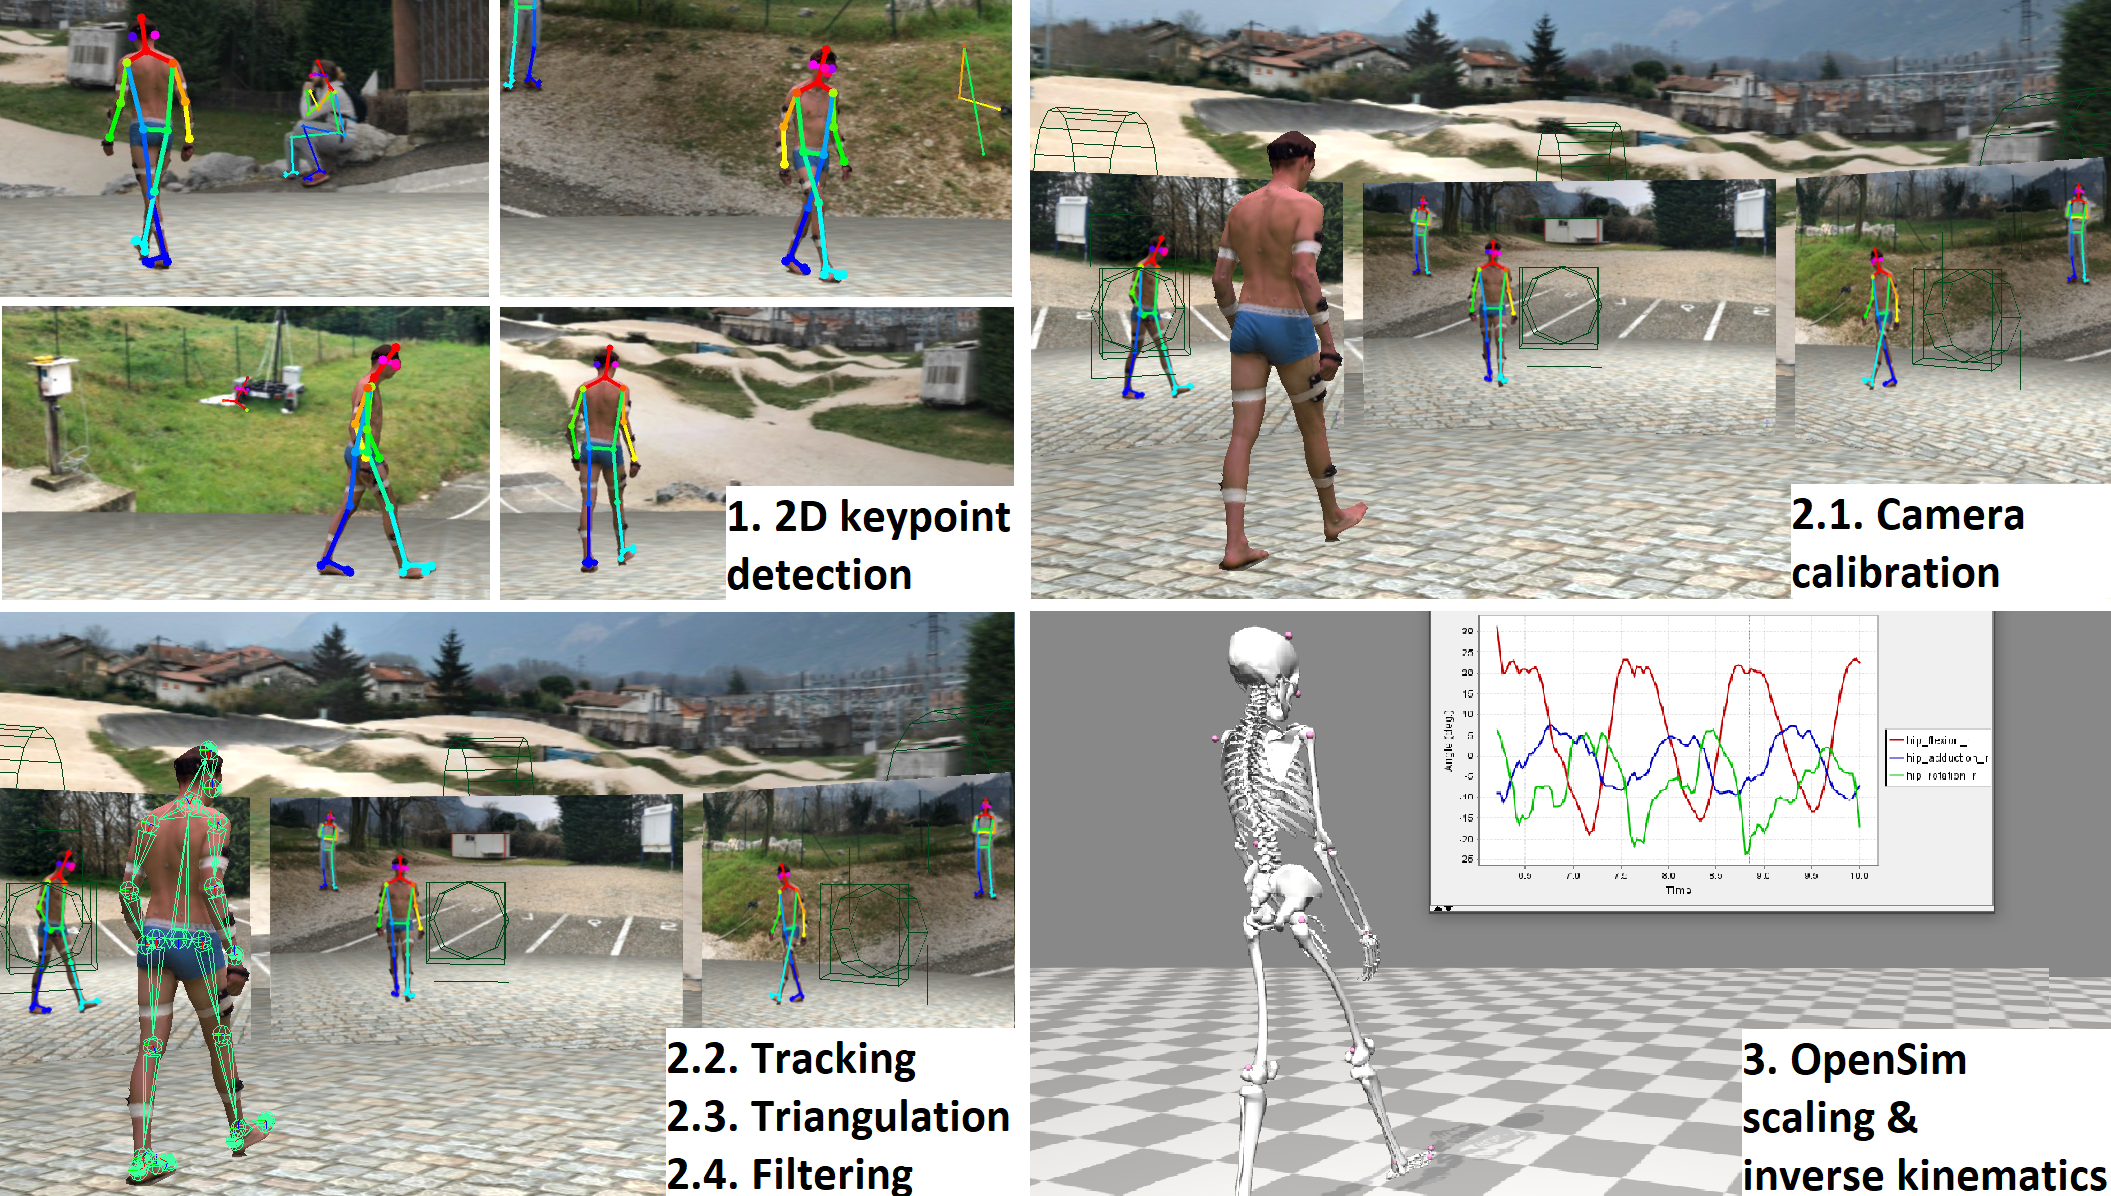
\includegraphics[width=\linewidth]{"../Chap3/Figures/Fig_Pipeline.png"}
	\caption{Pose2Sim full pipeline: (1) 2D keypoint detection; (2.1) Camera calibration; \newline(2.1-2.4) Tracking of the person of interest, Triangulating of keypoint coordinates; and Filtering; (3) Constraining the 3D coordinates to an individually scaled, physically consistent OpenSim skeletal model.}
	\label{fig_pipeline}
\end{figure}

\newpage

The repository presents a framework which consists in (see Figures~\ref{fig_pipeline} and \ref{fig_opensimutilities}):
\begin{enumerate}[itemsep=0em, topsep=0em, leftmargin=*]
      \item Preliminary 2D joint coordinate detections from multiple videos, e.g. with OpenPose.
      \item Pose2Sim core, including 4 customizable steps:
      \begin{enumerate}[before=\vspace{-0.5\baselineskip}, nosep, label*=\arabic*.]
            \item Camera calibration.
            \item 2D tracking of the person of interest.
            \item 3D keypoint triangulation.
            \item 3D coordinate filtering.
      \end{enumerate}
      \item Scaling a full-body skeleton to each individual subject, and computing inverse kinematics via OpenSim so as to obtain 3D joint angles.
\end{enumerate}

\vskip 1em

Pose2Sim requires only moderate Python skills, and each task is as fully and easily configurable as possible. By editing the \\\mintinline{shell-session}{User/Config.toml} file, the user can specify the project path and folder names, the video frame rate, the range of analyzed frames; as well as the 2D pose estimation model used, and calibration, tracking, and triangulation parameters. 

The whole workflow runs from any video cameras, on any computer, equipped with any operating system (although OpenSim has to be compiled from source on Linux). It requires no marker placement, and the scaling and inverse kinematic steps are simpler than they are with markers-based methods. Overall, human intervention is scarce, which makes it more robust to human error. Pose2Sim has already been used and tested in a number of situations (walking, running, cycling, dancing, balancing, swimming, boxing, BMX racing), and published in peer-reviewed scientific publications assessing the quality of its code \cite{Pagnon2022c}, its robustness (see Chapter 4 on \nameref{ch:4}) \cite{Pagnon2021} and its accuracy (see Chapter 5 on \nameref{ch:5}) \cite{Pagnon2022a}. Its results for inverse kinematics were deemed good when compared to marker-based ones, with errors generally below 4.0° across several activities, on both lower and on upper limbs. The combination of its ease of use, customizable parameters, and high robustness and accuracy makes it promising, especially for "in-the-wild" sports movement analysis.


\begin{figure}[hbtp]
	\centering
	\def\svgwidth{1\columnwidth}
	\fontsize{10pt}{10pt}\selectfont
	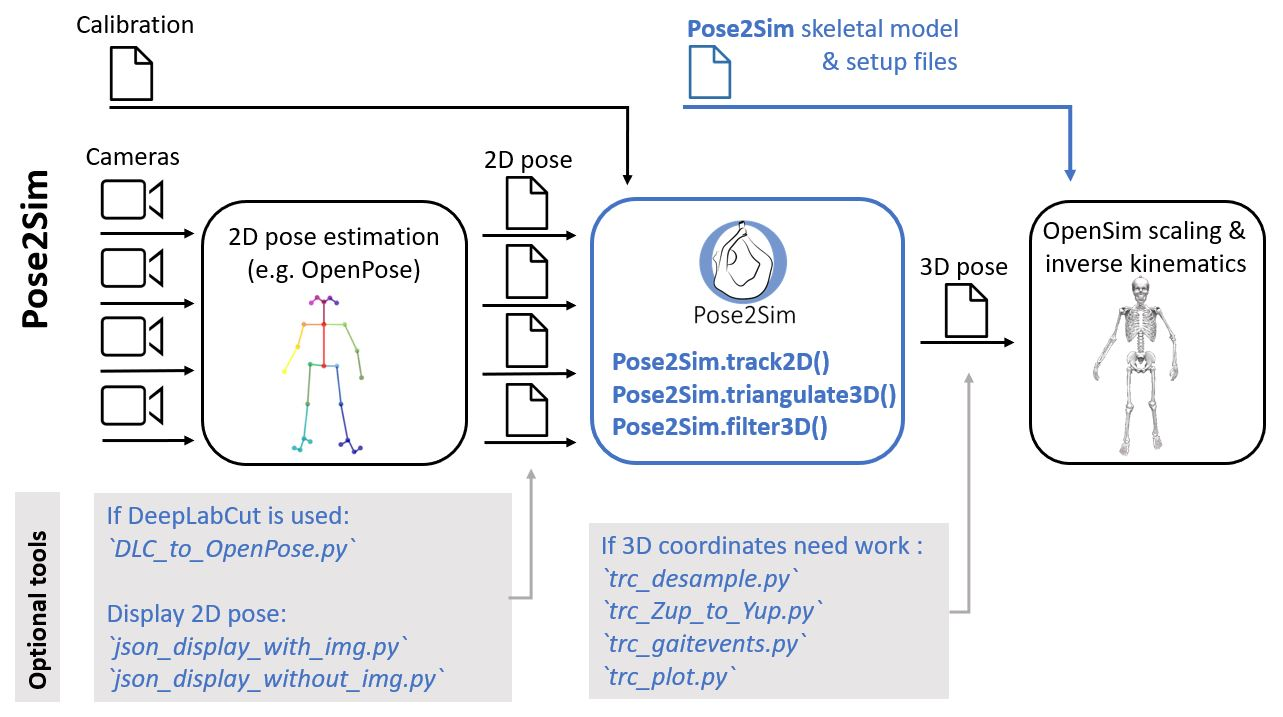
\includegraphics[width=\linewidth]{"../Chap3/Figures/Fig_Pose2SimUtilities.jpg"}
	\caption{The Pose2Sim workflow, along with some optional utilities provided in the package.}
	\label{fig_opensimutilities}
\end{figure}


\clearpage
\section{Method details}\label{methods_details}
\subsection{2D keypoint detection}

2D pose detection can be performed with any deep-learning pose estimation network and model. We recommend using the OpenPose body\_25B model, as it provides foot keypoints, is as fast as the standard body\_25 one, and as we have extensively tested it \cite{Pagnon2022a}. However, it requires manual installation \cite{Hidalgo2021}. Note that only 21 of the 25 detected keypoints are tracked, since eye and ear keypoints would be redundant in the determination of the head orientation. 

The choice of pose estimation model will affect how keypoint indices will be mapped to model markers in OpenSim, corresponding to anatomical landmarks or joint centers. The OpenPose body\_25, body\_25B, body\_135, COCO, and MPII models are fully supported. The AlphaPose COCO, COCO-WholeBody, and full-body HALPE models are also supported, as well as the full-body but single-person detection BlazePose model. COCO and MPII model are the ones generally used by other networks such as OpenPifPaf \cite{Kreiss2021}, YOLO-pose \cite{Maji2022, Wang2022b}, and others, which means that they are also supported. It is also possible to build custom skeletons in the \mintinline{shell-session}{skeleton.py} file, trained for example with DeepLabCut \cite{Mathis2018, Lauer2022} or SLEAP \cite{Pereira2022}. They will be triangulated, but the user will need to build an OpenSim skeletal model and set the keypoints in the right place before being able to perform inverse kinematics.

%%%%%%%%%%%%%%%%%%%%%%%%%%%%%%%%%%%%%%%%%%%%%%%%%%%%%%%%%%%%%%%%%%%
% ATTENTION:                                                      %
% IMPLEMENTER CES MODELES ET LES TESTER AVANT DE PUBLIER LA THESE %
%%%%%%%%%%%%%%%%%%%%%%%%%%%%%%%%%%%%%%%%%%%%%%%%%%%%%%%%%%%%%%%%%%%
% OpenPose body_25b, OpenPose body_25, OpenPose body_135, AlphaPose HALPE_26, AlphaPose HALPE_136, AlphaPose COCO-WholeBody, MediaPipe BlazePose, COCO, MPII
% Convert SLEAP to OpenPose

Two optional standalone scripts are also provided if the user desires a visual display of the 2D pose estimation, as well as a tool for converting DeepLabCut data to OpenPose formalism (Figure~\ref{fig_opensimutilities}).


\subsection{Camera calibration}

The user can indicate whether cameras are going to be calibrated with a checkerboard, or if a preexisting calibration file (such as one provided by a Qualisys system) will simply be converted.

If checkerboard calibration is chosen, the number of corners and the size of the squares have to be specified. In this case, the operator needs to take about 20 pictures or one video of the checkerboard per camera. Corners are then detected and refined with OpenCV \cite{Bradski2000}. Detected corners can optionally be displayed for verification. Each camera is finally calibrated using OpenCV based on an algorithm proposed by \cite{Zhang2000}. For intrinsic parameters' determination, the checkerboard needs to be taken from different angles, as close as possible to the camera, however without being cropped. For extrinsic parameters, only one frame is used. The checkerboard is classically laid flat on the ground, in a place visible by all cameras. The user can choose the index of the image which they want to be used as a reference for calculating extrinsic parameters. Residual calibration errors are given, and stored in a log file.


\subsection{Tracking the person of interest}\label{tracking}

One needs to differentiate the people in the background from the actual subject. The tracking step examines all possible triangulations of a chosen keypoint among all detected persons, and reprojects them on the image planes. The triangulation with the smallest reprojection error is considered to be the one associated with the right person on all cameras. If the reprojection error is above a predefined threshold, the process is repeated after taking off one, or several cameras. This happens, for example, if the person of interest has exited the field of a camera, while another person is still in the background.

We recommend choosing the neck point or one of the hip points. In most cases they are the least likely to move out of the camera views.


\subsection{Weighted triangulation}

Pose2Sim triangulation is robust, largely because instead of using classic Direct Linear Transformation (DLT) (see previous chapter on \nameref{triangulation}) like other approaches do \cite{Hidalgo2021,Matthis2022,Sheshadri2020,Easymocap2021}, we propose a weighted DLT, i.e., a triangulation procedure where each OpenPose keypoint coordinate is weighted with its confidence score \cite{Pagnon2021}. This is a good compromise between losing all confidence information, and triangulating the whole heatmap in a volumetric way \cite{Iskakov2019}, which is very slow. The weighted DLT has been independently introduced by \cite{Barone2020}, in the context of camera calibration. See Algorithm~\ref{alg:weighted_dlt} for the proposed solution. 

\begin{algorithm}[!ht]
      \caption{Weighted DLT}\label{alg:weighted_dlt}
      \begin{algorithmic}[1]
            \STATEx Our weighted DLT simply consists of weighing Equation~\ref{eq:factortrig} with the confidence c given by OpenPose for each camera. The rest of the procedure remains unchanged.
            \begin{equation}
                  \begin{cases}
                        &  c \times (\overrightarrow{P_1} - u_p \ \overrightarrow{P_3} ) \cdot \overrightarrow{Q_W}  = 0\\
                        &  c \times (\overrightarrow{P_2} - v_p \ \overrightarrow{P_3} ) \cdot \overrightarrow{Q_W}  = 0\\
                  \end{cases}
          \end{equation}
      \end{algorithmic}
\end{algorithm}

Other parameters can be specified, such as:
\begin{itemize}[itemsep=0em, topsep=0em, leftmargin=*]
      \item The minimum likelihood \(conf_{min}\) below which a 2D point will not be taken into account for triangulation. Each detected keypoint is attributed a confidence score by OpenPose.
      \item The maximum in reprojection error \(error_{max}\) above which triangulation results will not be accepted. This can happen if OpenPose provides a bad 2D keypoint estimate, or if the person of interest leaves the camera field. Triangulation will then be tried again on all subsets of all cameras minus one. If the best of the resulting reprojection errors is below the threshold, it is retained. If it is still above the threshold, one more camera is excluded.
      \item The minimum number of "good" cameras, \(ncams_{min}\) (i.e., cameras remaining after the last two steps) required for triangulating a keypoint. If there are not enough cameras left, the 3D keypoint is dropped for this frame.
\end{itemize}

See Algorithm~\ref{alg:pose2sim_trig} for the full algorithm of triangulation of a keypoint. Once all frames are triangulated, the ones with missing keypoint coordinates are interpolated. The interpolation method can also be chosen from among linear, slinear, quadratic, and cubic. The mean reprojection error over all frames is given for each point and saved to a log file, as well as the number of cameras excluded to reach the demanded thresholds. The resulting 3D coordinates are formatted as a .trc file, which is a tabulation-separated text format used by OpenSim.

If needed, other standalone tools are provided to further work on the .trc 3D coordinate files (Figure~\ref{fig_opensimutilities}). Among others, it is possible to undersample a file from a higher to a lower framerate, or to convert a file from Z-up to Y-up axis convention. The resulting 3D coordinates can be plotted for verification. Additionally, a tool is provided to detect gait events from point coordinates, according to the equations given by \cite{Zeni2008}.


\begin{algorithm}[!ht]
      \caption{Pose2Sim weighted triangulation of a keypoint}\label{alg:pose2sim_trig}
      \begin{algorithmic}[0]
            \STATE Let $error_{max}$ be the maximum allowed reprojection error, $ncams_{min}$ the minimum number of cameras demanded for triangulation (among $ncams_{tot}$ available cameras), and $conf_{min}$ the minimum confidence accepted for a keypoint to be used.
            \WHILE {$error > error_{max}$ AND $ncams > cams_{min}$}
                \FOR {all combinations $\binom{ncams_{tot}}{ncams}$}
                      \FOR {all cameras}
                        \IF {$conf>conf_{min}$}
                              \STATE $weighted\_DLT \gets add\_keypoint$
                        \ENDIF
                      \ENDFOR
                    \STATE $Q \gets solve\_weighted\_DLT$
                    \STATE $error \gets calculate\_reprojection\_error$
                \ENDFOR
                \IF {$min(error) < error_{max}$}
                    \STATE \textbf{return} $Q[min(error)], min(error)$
                \ELSE 
                    \STATE $ncams \gets ncams-1$
                \ENDIF                
            \ENDWHILE
      \end{algorithmic}
\end{algorithm}


\subsection{Filtering and other operations}

Different filters can be chosen, and their parameters can be adjusted. The user can choose a zero-phase low-pass Butterworth filter \cite{Butterworth1930} that they can apply either on keypoint positions or on their speeds, a LOESS filter \cite{Cleveland1981}, a Gaussian filter, or a median filter. We recommend choosing the first option, as it is the most customary method used in biomechanic sciences. Waveforms before and after filtering can be displayed and compared.



\subsection{OpenSim scaling and inverse kinematics}

OpenSim \cite{Delp2007,Seth2018} is a widespread open-source software which helps compute consistent 3D joint angles, usually from marker coordinates. It lets scientists define a detailed musculoskeletal model, scale it to individual subjects, and perform inverse kinematics. Results are accurate and robust since biomechanical constraints can be adjusted and weighted, bones are set to a constant length, and joints limited to coherent angle limits. OpenSim provides other features such as net calculation of joint moments or resolution of individual muscle forces, although this is beyond the scope of our contribution.

The main contribution of Pose2Sim is to build a bridge between OpenPose and OpenSim. The OpenSim model needs to be carefully crafted. Indeed, inverse kinematics is an under-constrained problem, that can be guided with carefully chosen joint constraints. Pose2Sim provides a full-body model, adapted from the human gait full-body model \cite{Rajagopal2016} and the lifting full-body model \cite{Beaucage-Gauvreau2019}. The first one has a better definition of the knee joint, with a coupling relationship between knee flexion and abduction/adduction and internal/external rotation. These joint constraints allow for reducing the 3D knee kinematics to a problem with only one degree of freedom, assuming that the observed individual does not bear any strong anatomical divergence to the norm. In the same way, the latter model has a better definition of the spine: each lumbar vertebra is constrained to the next one, which makes it possible for the spine to bend in a coherent way with only a few tracked keypoints, without having to make it a rigid single bone. Combining those two models allows for ours to be as versatile as possible. Hand movements are locked, because the standard OpenPose models don't provide any hand detection. A ball joint was added between head and torso so that the rotation of the head could be roughly rendered. Of course, the user can also build their own OpenSim model, and use the markerset of their choice.

The placement of markers on the model is also of paramount importance, especially with so little of them. OpenPose keypoints do not necessarily coincide with joint centers, probably because of systematic labelling errors in the training dataset \cite{Needham2021b}. Moreover, they may be located in a different anatomical position when limbs are fully extended in comparison to when they are fully flexed. However, once model markers are positioned in accordance with those of the triangulated 2D pose estimations, the scaling step is very fast and straightforward since the marker placement will not change from one session, subject, or operator to another. Our model takes these labelling errors into account, and offsets model markers as regards true joint centers accordingly (Figure~\ref{fig_mkmkl}).

\begin{figure}[!ht]
	\centering
	\def\svgwidth{1\columnwidth}
	\fontsize{10pt}{10pt}\selectfont
	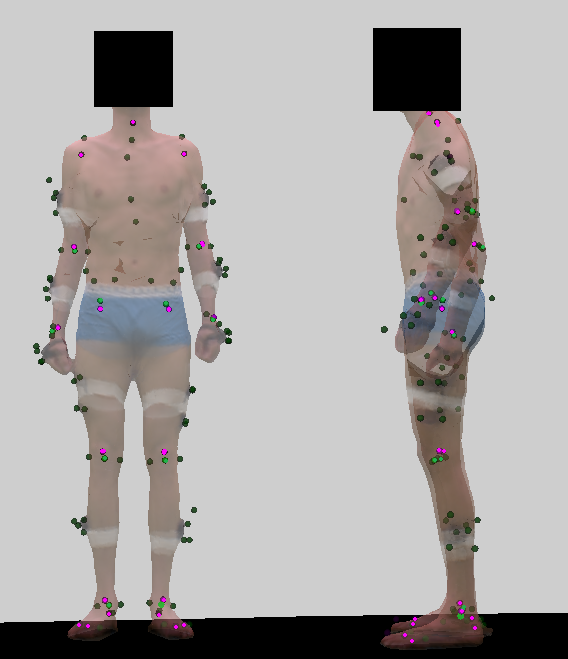
\includegraphics[width=.95\linewidth]{"../Chap3/Figures/Fig_MkMkl.png"}
	\caption{Triangulated anatomical markers and clusters (dark green), calculated joint centers (light green), and OpenPose body\_25B keypoints (pink) on a textured mesh. OpenPose’s eyes and ears keypoints were excluded. Mesh opacity was set to 0.5 in order to make all points visible. This view made it possible to precisely place OpenPose triangulated keypoints on the OpenSim model.}
	\label{fig_mkmkl}
\end{figure}

Scaling in OpenSim can be broken down into two parts: first, the proper scaling of the model, which adjusts bone dimensions and inertial properties according to the distances between the joint markers; second, the adjustment of the other markers on the model, especially anatomical and cluster markers. Joint centers are not trivial to obtain in marker-based approaches, since they must be calculated from the position of skin markers or from clusters: this is not an issue for OpenPose triangulated keypoints, which already represent joint centers in the first place. Moreover, if the model is defined properly, there is no need for further marker adjustment, since markers will not be subject to placement variation due to human error or to skin movement artifacts. Hence, only the first step of scaling must be undergone, and it is simpler than in marker-based approaches. Each body is scaled according to a factor computed as a ratio of distances, defined by the distance between pairs of model markers over distance between corresponding pairs of experimental markers. The markers used for scaling are chosen as follows:

\begin{itemize}[itemsep=0em, topsep=0em, leftmargin=*]
      \item{Arm: distance between shoulder and elbow markers;}
      \item{Forearm: distance between elbow and wrist;}
      \item{Thigh: distance between hip and knee;}
      \item{Shank: distance between knee and ankle;}
      \item{Foot: distance between heel and big toe;}
      \item{Pelvis: distance between left and right hip;}
      \item{Torso: distance between neck and hip;}
      \item{Head: distance between head and nose;}
\end{itemize}
All weights of joint coordinates are set to 1, apart from those of the nose and the head, which are set to 0.2, and from those of the other head markers, which are set to 0. We recommend scaling on a standing pose, which is easy to keep for a second, usually not too far from sports poses, and accurately estimated by 2D pose detection models. Moreover, if this condition is satisfied, we can add as a scaling assumption that ankle flexion should be fixed at a neutral 0° angle. 

The inverse kinematic tool is used with the same marker weights as in the scaling step. Unlike in marker-based capture, keypoints detection hardly depends on the operator, the subject, nor the context. For this reason, the scaling and the inverse kinematic steps are straightforward, and the provided setup files require little to no adjusting.


\subsection{Other features}

Optional tools are also provided for extending its usage (Figures~\ref{fig_opensimutilities}). Among others, DeepLabCut 2D files can be converted to the OpenPose formalism, and calibration files from other platforms can also be converted to the AniPose \cite{Karashchuk2021} formalism we use. 2D keypoint files can be displayed and stored as a video. Gait events can be detected from kinematic data thanks to \cite{Zeni2008} algorithm. Some other scripts allow for further processing of 3D coordinates. More practical information can be found on the GitHub repository. 


\section{Limits and perspectives} \label{ch3_lim}

\subsection{2D keypoint detection}

Pose2Sim is currently primarily used with OpenPose as a 2D pose detection network. Despite it is very robust, it suffers from issues when used for full-body kinematic analysis. First, keypoint localization suffers from systematic offsets when compared to actual joint center positions \cite{Needham2021b}. Constraining these coordinates to a skeletal model largely reduces the detrimental impact of low-quality 2D joint center estimations. Nevertheless, these offsets have been taken into account in the provided OpenSim model, by shifting OpenPose keypoint placements with regard to marker-based calculated joint centers. This was done manually, but precisely, thanks to our overlayed view (Figure~\ref{fig_mkmkl}). However, OpenPose’s offset may not be the same when a limb is extended as when it is bent, which may influence kinematic results on extreme poses, such as observed in some sports disciplines. Hence, using a 2D pose estimation model free from systematic biases on all ranges of motion would certainly improve kinematic accuracy. The body\_25B model is more accurate than the default body\_25 one, but it is still biased. 

Furthermore, both models only detect 25 keypoints. This makes inverse kinematics an under-constrained problem, which has to be guided with carefully chosen joint constraints, and with precise placement of markers on the model. Currently, all pelvis, lumbar, and thoracic angles are solely determined by the detection of the hip keypoints on the lower part, and of the shoulder and neck keypoints on the upper part. As a consequence, even if joint centers were perfectly estimated, the optimization procedure would admit two solutions for the spine curvature, both mathematically and kinematically correct: one with a lordotic posture, and the other with a kyphotic posture. Additionally, there is no marker for the hand, which does not allow for capture of any pronation/supination movement, let alone of any hand or finger movement. The shoulder is also defined as a ball joint, whereas the pectoral girdle is much more complex. Internal/external rotations are solved with difficulties despite the use of kinematic constraints. Using the experimental body\_135 OpenPose model would solve the hand issue, but it would also greatly increase the computational cost and would leave the shoulder and spine problem unaddressed. As a consequence, and provided that they are reliably labeled, OpenPose needs more keypoints to solve these indeterminations, and potentially several per joints, in the same way as markersets are designed in marker-based methods. Pose2Sim could operate with such a model, although new keypoints should then be placed afresh on the unscaled OpenSim model. 

Moreover, OpenPose struggles to accurately detect pose when the person taking an unusual pose. One way to solve this is by enhancing the OpenPose dataset, by augmenting it with larger image rotations so that upside-down poses are recognized, or by training it on specific sports poses. One risk of this approach is that the model may perform better on specific extreme poses, but worse on standard ones \cite{Kitamura2022}. As a consequence, it could be interesting to build a new dataset, with more accurate labelling, more keypoints, trained on specific sports poses.

On a different note, in a sports context, not only the human pose is of interest: sports gear can also be considerably important to detect, such as a ball \cite{Ghasemzadeh2021}, skis \cite{Ludwig2020}, or bike parts in the context of cycling (see \autoref{ch:7} on  \hyperref[ch:7]{Capturing equipment along with the athlete}). This can help to analyze game dynamics, and to quantify posture cues related to a specific sports discipline. This can be done, for example, by separately process human pose with OpenPose, and equipment pose with a custom-trained DeepLabCut model. Resulting .trc coordinate files can be merged, and used in OpenSim. However, the DeeLabCut keypoints must be referenced on an OpenSim model, which will need to be crafted from scratch.


\subsection{User-friendly calibration and triangulation options}

Calibration remains a challenging task in broad daylight, at a distance, and with non research-grade cameras. It could be useful to make it more robust, either by implementing the Aniposelib library \cite{Karashchuk2020}, by importing calibration files from an Argus wand calibration \cite{Argus}, or by automatically calibrating on people’s limb length \cite{Liu2022a}. Overall, numerous other calibration and triangulation approaches have been proposed in the literature and could be implemented (see \autoref{ch:2}). Along with synchronization of light-weight cameras, a practical issue and its resolution is detailed in \autoref{ch:6} on \hyperref[ch:6]{Key Performance Indicator assessment with action cameras} \cite{Pagnon2022c}. 


\subsection{Multi-person analysis}

Despite it is not altered by people entering the field of view, Pose2Sim can currently only analyze the movement of one single person. For races, team sports, and combat sports, it would be useful to be able to analyze the movement of several athletes at the same time. This could be achieved in two steps: first, by triangulating all the persons whose reprojection error is below a certain threshold, instead of taking only the one with minimum error, in a similar way as carried out by \cite{Slembrouck2020}; then, by tracking the triangulated persons in time, e.g., by limiting the displacement speed of each person’s neck keypoint from one frame to the next one (see \nameref{triangulation} in previous chapter for more insight on available methods). 


\subsection{Real-time analysis}\label{subsec:realtime}

Currently, Pose2Sim does not work in real time. This is a drawback for coaches and athletes, who need feedback in a timely manner. However, a timely analysis of athletes’ movements directly on the sports field appears to be achievable. Indeed, OpenPose is faster than most of its competitors \cite{Chen2020a}, and the rest of the process is not computationally costly. Moreover, the pose detection, the triangulation, and the OpenSim inverse kinematic optimization work frame by frame. As a consequence, it is conceivable to calibrate and scale the model first, and then to feed the GUI frame by frame. This would allow the workflow to operate with only a few seconds of delay.


\subsection{Visualization tools}\label{subsec:viztools}

Pose2Sim does not provide a GUI yet. This can make it complicated for coaches to adopt the tool. However, the code has been adopted by other entities. The 3D animation "CEB" studio built a Blender \cite{Blender1998} extension using Pose2Sim for realistic 3D markerless animation. However, it is not free nor open-source \cite{Barreto2022} (Figure~\ref{fig_mpp2sos}). In addition, the CAMERA laboratory of the University of Bath is currently developing a GUI around Pose2Sim, which would make the tool more accessible. 

\begin{figure}[hbtp]
      \centering
      \def\svgwidth{1\columnwidth}
      \fontsize{10pt}{10pt}\selectfont
      \href{https://blendermarket.com/products/mocap-mpp2soss}{
            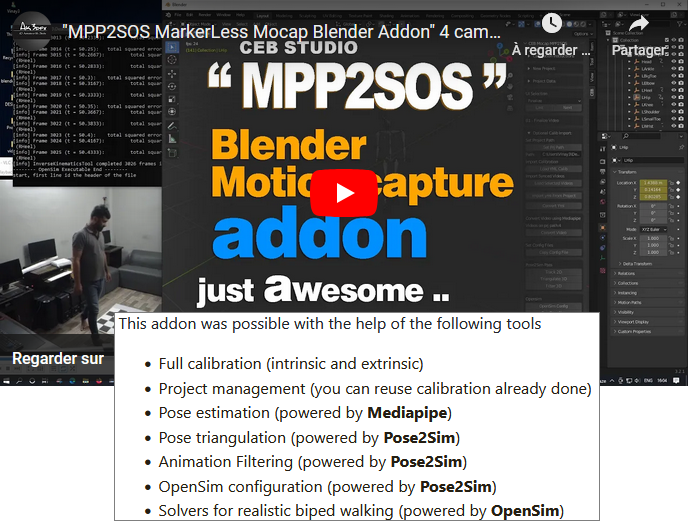
\includegraphics[width=1\linewidth]{"../Chap3/Figures/Fig_MPP2SOS.png"}
      }
      \caption{CEB Studio built the MPP2SOS Blender add-on, which uses Pose2Sim for realistic 3D markerless animation.}
      \label{fig_mpp2sos}
\end{figure}

\begin{figure}[h!]
	\centering
	\begin{subfigure}[b]{1\textwidth}
		\centering
		\def\svgwidth{\columnwidth}
		\fontsize{10pt}{10pt}\selectfont
		\href{https://github.com/davidpagnon/Maya-Mocap}{
                  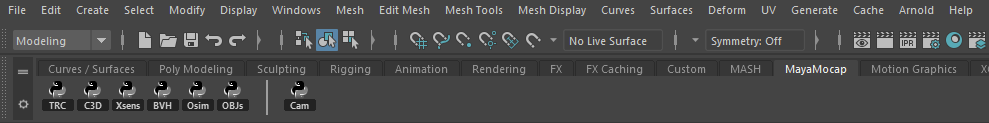
\includegraphics[width=\linewidth]{"../Chap3/Figures/Fig_MayaMocap1.png"}
            }
            \caption{The Maya-Mocap add-on is displayed as an additional toolbar in Maya.}
      \end{subfigure}
	\qquad
	\begin{subfigure}[b]{1\textwidth}
		\centering
		\def\svgwidth{\columnwidth}
		\fontsize{10pt}{10pt}\selectfont
		\href{https://github.com/davidpagnon/Maya-Mocap}{
                  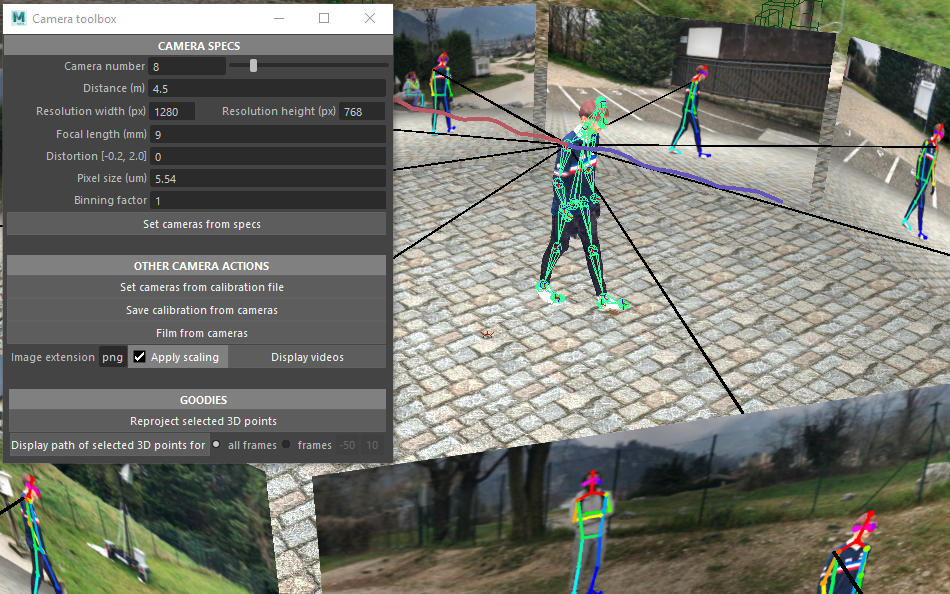
\includegraphics[width=\linewidth]{"../Chap3/Figures/Fig_MayaMocap2.png"}
            }
            \caption{Maya-Mocap can import several file types, e.g., a .trc motion file (bright green) or a textured animated 3D mesh. It can also load cameras from a calibration file, film with them, and display the filmed image sequences. In addition, it can reproject a selected point onto the camera plane (black lines), to make sure that it has been correctly triangulated. The 3D trajectory of a point can also be highlighted (red and blue lines).}
      \end{subfigure}
      \caption{The Maya-Mocap add-on}
	\label{fig_mayamocap}
\end{figure}

I also developed a toolbox for Maya \cite{Maya1998} called Maya Mocap \cite{Pagnon2020}. First, it can import and display various types of motion files. Then, it can load cameras from a calibration file, film with them, and import the filmed image sequences. It can also help to make sure that triangulated points are well reprojected on the camera plane, by tracing a line from the point to the camera center. In addition, it can display the 3D trajectory of a point (see Figure~\ref{fig_mayamocap}). Next objectives would be to make it able to import an OpenSim model and its motion files, and to present it as a cleaner package, ready to be released. Since all the tools used in Pose2Sim are open-source, it would also be more consistent to translate it into Blender instead of Maya, in order to offer an entirely operational and open-source tool.


\FloatBarrier
\subsection{Other perspectives}

Other minor adjustments could be made in order to improve the workflow or to give it more options. Other calibration, triangulation, or filtering methods could be implemented. Opting for an optimal fixed-interval Kalman smoother instead of a low-pass Butterworth filter \cite{Rauch1965,Needham2021a} may reduce errors, especially in large outliers. However, since a Kalman smoother works on all frames of a signal, it would make real-time analysis impossible. Instead of constraining 3D pose estimation results with a physically consistent skeletal model, it would be interesting to develop a physics-informed 2D pose estimation model \cite{Raissi2019,Xu2020a}, which would offer the opportunity of embedding the kinematics priors as early as possible in the learning process, or conversely as a refinement step upon triangulation \cite{Hua2022}. Adding muscles which were stripped from the skeleton in the OpenSim model could allow for joint kinetics prediction. Neural networks could be trained to estimate ground reaction forces from kinematics on specific tasks, without the use of a force platform \cite{Oh2013,Johnson2018,Mundt2019}. Performing pose estimation, robust triangulation, and inverse kinematics on the cloud rather than on a local computer could allow athletes and coaches to use the software in a web application. Nevertheless, local regulations such as the European GDPR should be respected. 

